%!TEX root = ../template.tex
%%%%%%%%%%%%%%%%%%%%%%%%%%%%%%%%%%%%%%%%%%%%%%%%%%%%%%%%%%%%%%%%%%%%
%% appendix-cascade.tex
%% Resolution cascade sequence diagrams (ported from ISEL-Thesis-2526/thesis/appendix.tex)
%%%%%%%%%%%%%%%%%%%%%%%%%%%%%%%%%%%%%%%%%%%%%%%%%%%%%%%%%%%%%%%%%%%%
\chapter{Resolution Cascade Sequence Diagrams}
\label{app:cascade-sequences}

This appendix collects the sequence diagrams supporting the discussion of the two provider
resolvers in \S\ref{subsec:store-internals}, one per level of the resolution cascade
(\S\ref{sec:resolution-cascade}), each contrasting the GCP and AWS behaviour side by side.

\begin{figure}[htb]
  \centering
  \begin{minipage}[t]{0.48\textwidth}
    \centering
    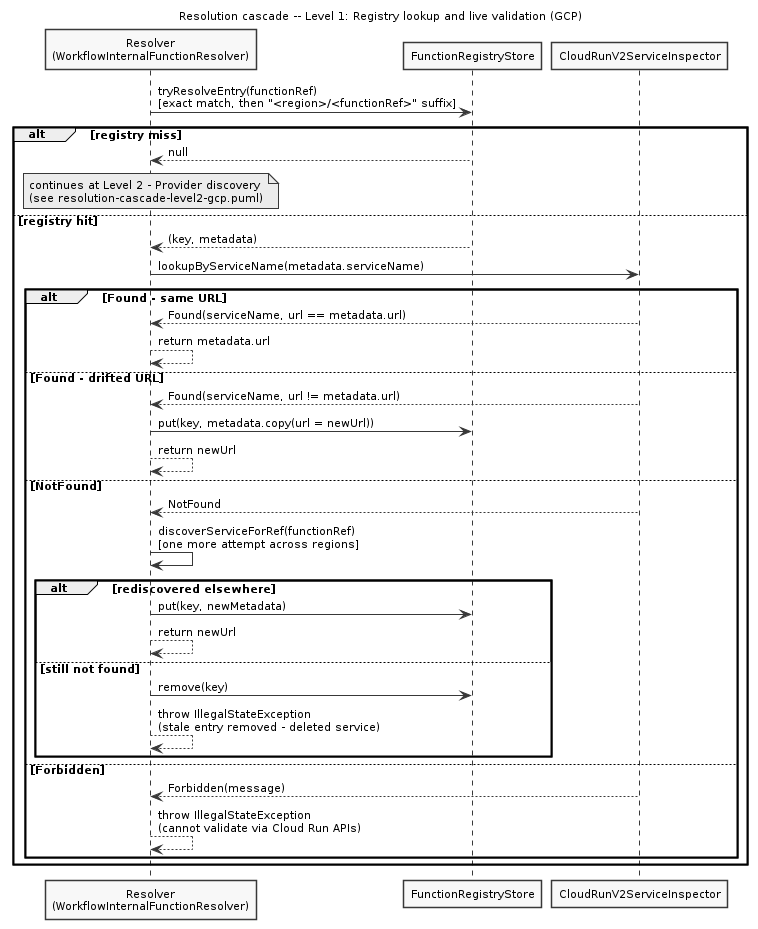
\includegraphics[width=\textwidth]{images/implementation/resolution-cascade-level1-gcp.png}
    \par (a) GCP
  \end{minipage}
  \hfill
  \begin{minipage}[t]{0.48\textwidth}
    \centering
    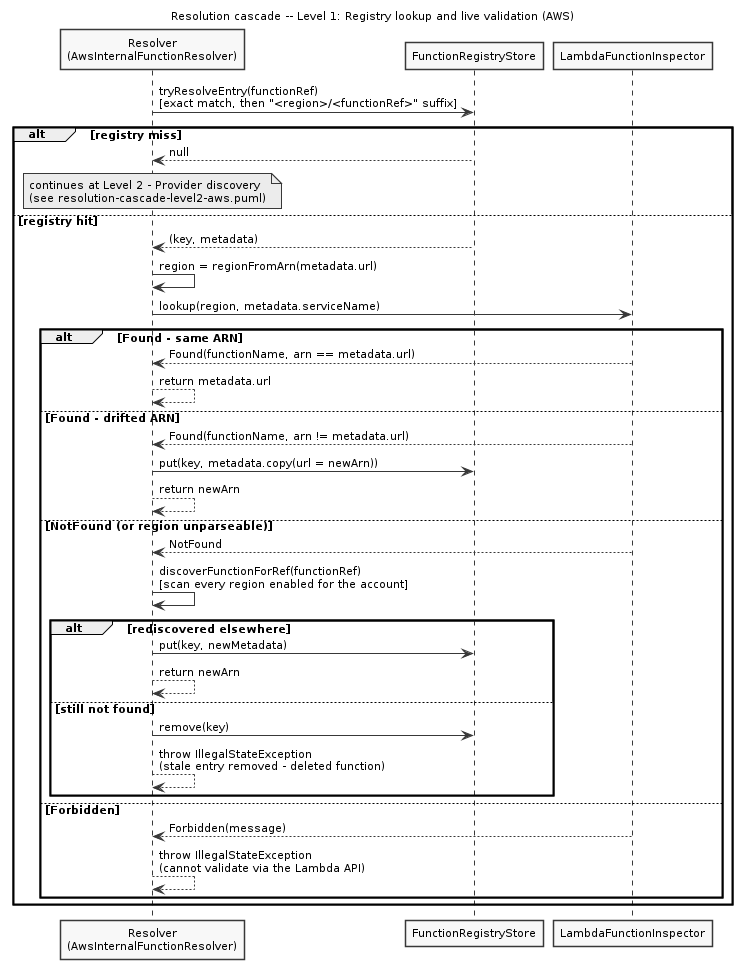
\includegraphics[width=\textwidth]{images/implementation/resolution-cascade-level1-aws.png}
    \par (b) AWS
  \end{minipage}
  \caption{Level~1 (Registry): a registry hit is validated against the live Cloud Run service on
  GCP (a) and against \texttt{GetFunction} on AWS (b); on a \texttt{NotFound} result, both paths
  attempt rediscovery across every region before a stale entry is removed. On GCP, bindings to
  first-generation Cloud Functions skip this validation (\S\ref{subsec:store-internals}).}
  \label{fig:resolution-cascade-level1}
\end{figure}

\begin{figure}[htb]
  \centering
  \begin{minipage}[t]{0.48\textwidth}
    \centering
    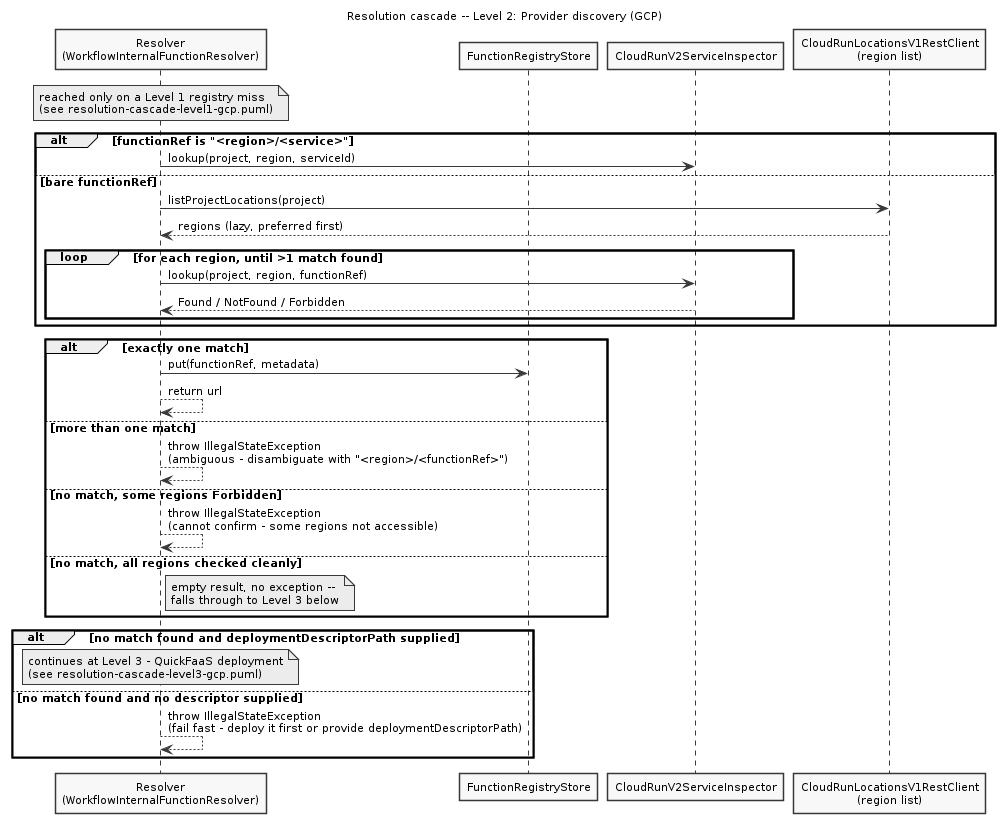
\includegraphics[width=\textwidth]{images/implementation/resolution-cascade-level2-gcp.png}
    \par (a) GCP
  \end{minipage}
  \hfill
  \begin{minipage}[t]{0.48\textwidth}
    \centering
    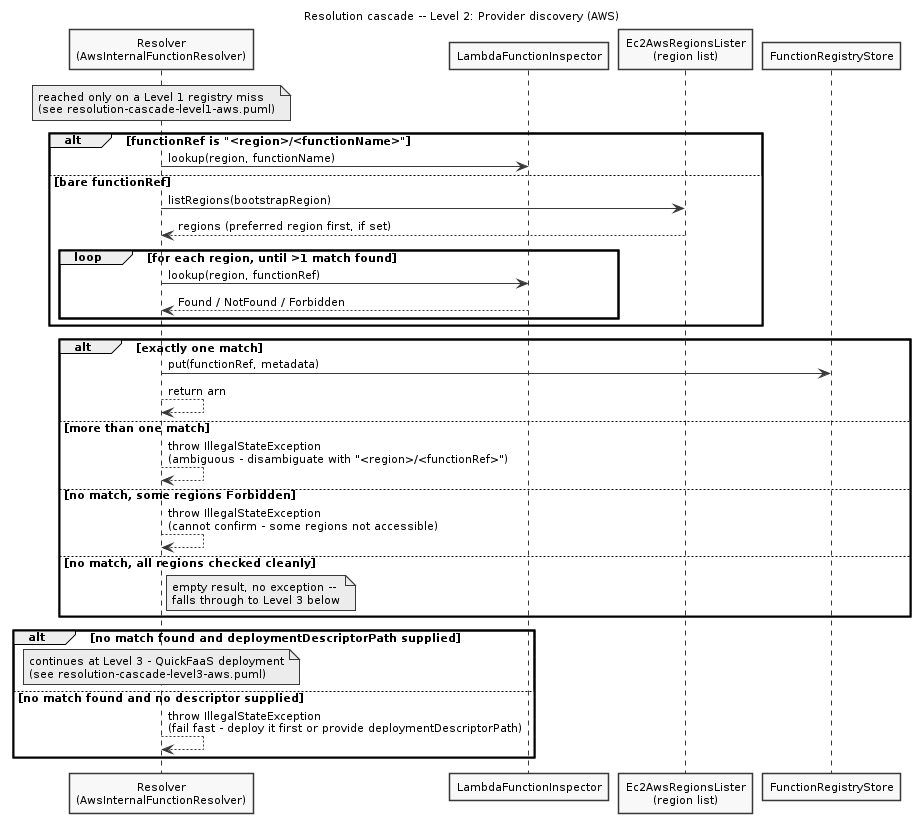
\includegraphics[width=\textwidth]{images/implementation/resolution-cascade-level2-aws.png}
    \par (b) AWS
  \end{minipage}
  \caption{Level~2 (Provider discovery): the target Cloud Run service is searched for across the
  project's regions on GCP (a); the target Lambda is searched for across every region enabled for
  the account on AWS (b), or resolved with a single \texttt{GetFunction} call when the
  fully-qualified \texttt{"region/functionRef"} form is used.}
  \label{fig:resolution-cascade-level2}
\end{figure}

\begin{figure}[htb]
  \centering
  \begin{minipage}[t]{0.48\textwidth}
    \centering
    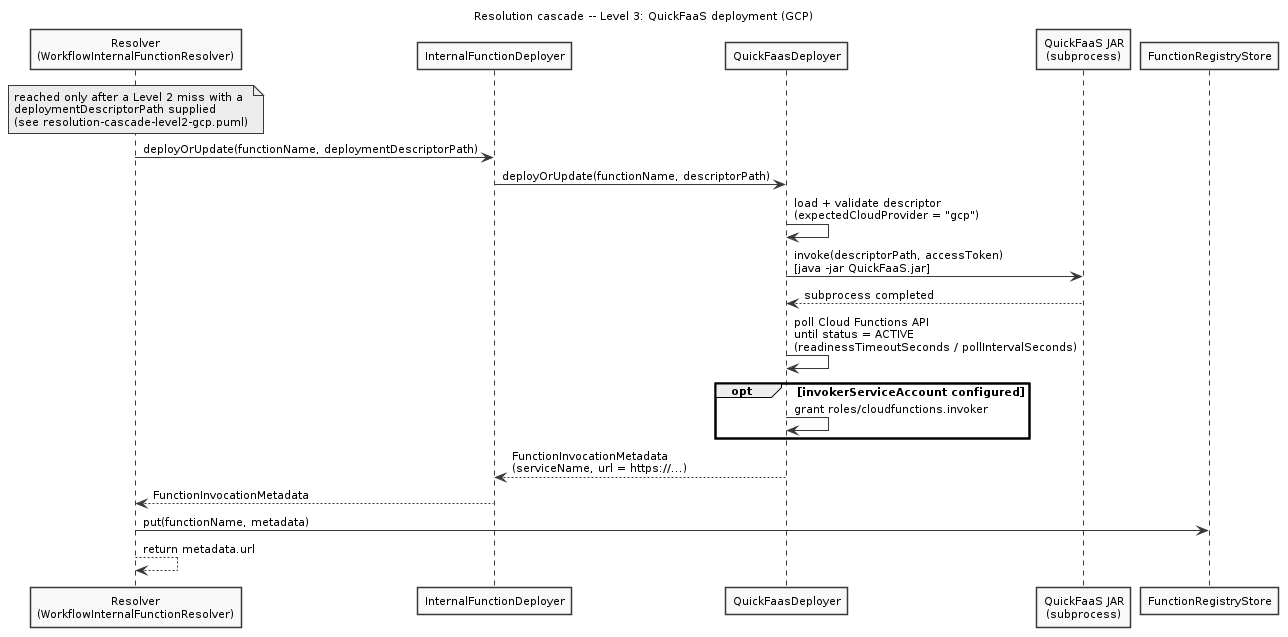
\includegraphics[width=\textwidth]{images/implementation/resolution-cascade-level3-gcp.png}
    \par (a) GCP
  \end{minipage}
  \hfill
  \begin{minipage}[t]{0.48\textwidth}
    \centering
    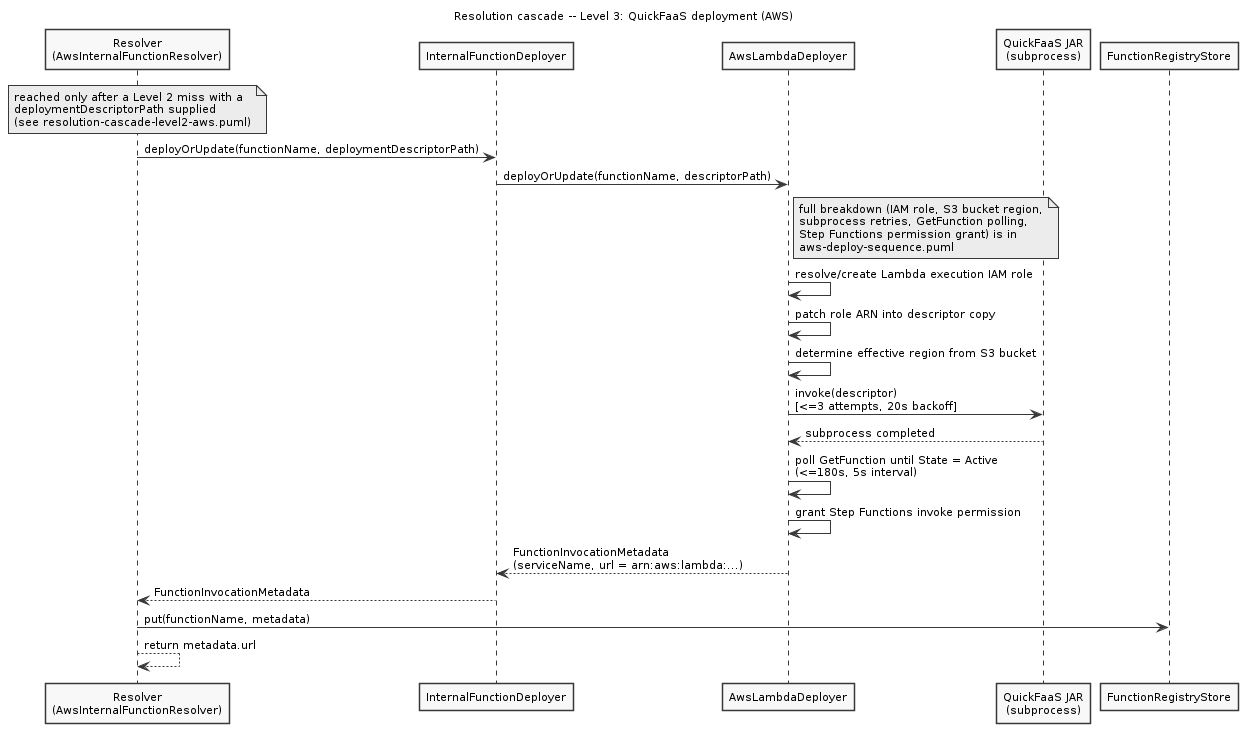
\includegraphics[width=\textwidth]{images/implementation/resolution-cascade-level3-aws.png}
    \par (b) AWS
  \end{minipage}
  \caption{Level~3 (QuickFaaS deployment): \texttt{QuickFaasDeployer} invokes QuickFaaS and polls
  the Cloud Functions API until the function is active on GCP (a); \texttt{AwsLambdaDeployer}
  invokes QuickFaaS and polls \texttt{GetFunction} until the Lambda is active on AWS (b).}
  \label{fig:resolution-cascade-level3}
\end{figure}
